% ============================================================
%  Quantum Effects in Biological Computing:
%  A Computational Investigation of Neural Transport,
%  Coherence, and Reservoir Capacity
% ============================================================
\documentclass[twocolumn,11pt]{article}

\usepackage{graphicx}
\usepackage{hyperref}
\usepackage{xcolor}
\usepackage{booktabs}
\usepackage{siunitx}
\usepackage{amsmath,amssymb}
\usepackage[numbers,sort&compress]{natbib}
\usepackage[margin=2cm]{geometry}
\usepackage{abstract}
\usepackage{orcidlink}
\usepackage[blocks]{authblk}

\sisetup{
  separate-uncertainty = true,
  multi-part-units     = single,
}

\hypersetup{
  colorlinks = true,
  linkcolor  = blue!60!black,
  citecolor  = blue!60!black,
  urlcolor   = blue!60!black,
}

% Short-hands
\newcommand{\kB}{k_{\mathrm{B}}}
\newcommand{\gamcm}{\gamma\;[\si{cm^{-1}}]}
\newcommand{\MC}{\mathrm{MC}}
\newcommand{\ENAQT}{\mathrm{ENAQT}}
\newcommand{\Pfour}{P_{4}}
\newcommand{\CVISI}{C_{\!V,\mathrm{ISI}}}

\begin{document}

% ============================================================
\title{Quantum Effects in Biological Computing:\\
  A Computational Investigation of Neural Transport,\\
  Coherence, and Reservoir Capacity}

\author{Celal Arda \orcidlink{0009-0006-4563-8325}}
\affil{Independent Researcher}
\affil{\texttt{celal.arda@outlook.de}}

\date{\today}

\twocolumn[
  \begin{@twocolumnfalse}
  \maketitle
  \begin{onecolabstract}
Whether quantum-mechanical effects play a functional role in
warm, wet neural tissue remains one of the most contested
questions in biophysics.
We report five computational experiments that systematically
investigate the hypothesis that quantum phenomena---tunnelling
delays, nuclear-spin coherence, and environment-assisted quantum
transport (ENAQT)---can enhance neural computation.

Using spiking-network simulations (BRIAN2), open-quantum-system
dynamics (QuTiP), and echo-state networks (ESN), we find:
(i)~quantum-tunnelling synaptic delays increase the coefficient
of variation of inter-spike intervals by 44\% and the Fano factor
by 89\% compared to classical fixed delays;
(ii)~$^{31}$P nuclear-spin coherence in a Posner-molecule model
survives \SI{346}{\micro\second} at body temperature
(\SI{310}{\kelvin});
(iii)~a 4-site ion-channel model exhibits an ENAQT peak at
$\gamma \approx \SI{1145}{cm^{-1}}$ with a 6.7$\times$
enhancement over the coherent limit;
(iv)~quantum-distributed noise preserves reservoir memory
capacity (MC) better than Gaussian noise at high amplitudes;
and (v)~when the ENAQT transport efficiency $\Pfour$ is used
as the synaptic release probability in an ESN, the MC peak
coincides \emph{exactly} with the ENAQT peak
($\gamma = \SI{1061}{cm^{-1}}$), demonstrating that
quantum-enhanced molecular transport directly translates into
quantum-enhanced network computation.

These results establish a quantitative bridge between
sub-molecular quantum effects and network-level computational
capacity, and generate falsifiable predictions for future
wet-lab organoid experiments.
  \end{onecolabstract}
  \vspace{1em}
  \end{@twocolumnfalse}
]

% ============================================================
\section{Introduction}
\label{sec:intro}

Biological computing---growing living neurons on silicon chips
and exploiting their self-organising dynamics for information
processing---has advanced from laboratory curiosity to early
commercial reality~\cite{Kagan2022,Smirnova2023,Cai2023}.
In~2022 the DishBrain system demonstrated that
\textit{in vitro} cortical neurons learn to play Pong with
higher sample efficiency than deep reinforcement
learning~\cite{Kagan2022}.  By~2023 brain-organoid cultures
solved reservoir-computing benchmarks~\cite{Cai2023}.
These platforms operate at body temperature (\SI{37}{\celsius})
in aqueous ionic media---conditions widely assumed to be hostile
to quantum coherence~\cite{Tegmark2000}.

Yet several lines of evidence challenge this assumption.
Photosynthetic antenna complexes sustain excitonic coherence for
hundreds of femtoseconds at ambient temperature, and
environment-assisted quantum transport (ENAQT) has been shown to
\emph{enhance} energy-transfer efficiency beyond both the
fully coherent and fully incoherent
limits~\cite{Engel2007,Mohseni2008,Plenio2008,Rebentrost2009}.
Cryptochrome proteins in migratory birds maintain entangled
radical-pair states for microseconds at \SI{41}{\celsius}, enabling
a biological compass~\cite{Xu2021}.
Enzyme-active sites exploit proton tunnelling for catalytic
rate enhancement~\cite{Scrutton2012}.
Fisher has argued that $^{31}$P nuclear spins in
calcium-phosphate Posner molecules could act as long-lived
quantum memory in the brain~\cite{Fisher2015}.

These observations share a common architectural motif: a
\emph{protein fold} or \emph{molecular cage} that shields a
nanoscale quantum-coherent domain from the thermal environment
just long enough for the quantum effect to be functionally
useful~\cite{Lambert2013,Cao2020,Kim2021}.
We term this the ``quantum ridge''---the boundary between
quantum and classical regimes where biology appears to extract
computational advantage.

The present work asks a specific, quantitative question:
\emph{Does quantum-enhanced molecular transport translate into
enhanced network-level computation?}
We approach this through five computational experiments that
build progressively from single-neuron effects (Experiment~1a)
through molecular-scale quantum dynamics (1b,~1c) to
network-level computational capacity (1d,~1e).  The final
experiment bridges quantum ion-channel transport and reservoir
computing in a single integrated model.

% ============================================================
\section{Methods}
\label{sec:methods}

All simulations use Python~3.11 with BRIAN2~\cite{Stimberg2019}
for spiking-network models and
QuTiP~\cite{Johansson2012,Johansson2013} for open-quantum-system
dynamics.  Code and data are available at
\url{https://github.com/[redacted]/Biological-Computing}.

% ---- 1a -----------------------------------------------------
\subsection{Experiment 1a: Quantum-modified synaptic delays}
\label{sec:meth-1a}

A recurrent spiking network of $N = 1000$ leaky integrate-and-fire
(LIF) neurons (800 excitatory, 200 inhibitory) is simulated
for \SI{2}{\second} with random connectivity ($p = 0.1$).
Two conditions are compared:

\begin{itemize}
  \item \textbf{Classical}: fixed synaptic delay
    $d_{\mathrm{cl}} = \SI{1.5}{\milli\second}$.
  \item \textbf{Quantum}: delay drawn from a
    tunnelling-modified distribution with mean
    $\langle d_{\mathrm{q}} \rangle = \SI{3.93}{\milli\second}$,
    $\sigma = \SI{0.35}{\milli\second}$, derived from a
    WKB tunnelling probability through a
    \SI{0.3}{\electronvolt} barrier.
\end{itemize}

Metrics: spike count, mean firing rate, coefficient of variation
of inter-spike intervals ($\CVISI$), Fano factor, and
spike-train entropy.

% ---- 1b -----------------------------------------------------
\subsection{Experiment 1b: Posner~$^{31}$P spin dynamics}
\label{sec:meth-1b}

A 6-spin model of $^{31}$P nuclei in a Posner molecule
($\mathrm{Ca_9(PO_4)_6}$) is evolved under a Lindblad master
equation.  The Hamiltonian includes Zeeman splitting in Earth's
magnetic field ($B = \SI{50}{\micro\tesla}$, Larmor frequency
\SI{862.6}{\hertz}) and dipolar couplings between spin pairs at
realistic inter-phosphorus distances
(\SIrange{4.0}{5.5}{\angstrom}).

Decoherence is modelled by pure dephasing ($\gamma_2$) and
longitudinal relaxation ($T_1$).
We sweep $\gamma_2$ from \SI{10}{\hertz} to \SI{e6}{\hertz}
and map temperature (\SIrange{4}{310}{\kelvin}) to dephasing
rate via $\gamma_2 = \kB T / (\hbar \cdot T_1)$ with
$T_1 = \SI{5}{\second}$ at body temperature.

Coherence time $\tau_c$ is defined as the $1/e$ decay time
of $|\langle \hat{\sigma}_x \rangle|$.

% ---- 1c -----------------------------------------------------
\subsection{Experiment 1c: ENAQT in a model ion channel}
\label{sec:meth-1c}

A 4-site tight-binding chain models single-file ion transit
through a selectivity filter (total length \SI{12}{\angstrom}).
The Hamiltonian reads
\begin{equation}
  \hat{H} = J \sum_{i=1}^{3} \bigl(|i\rangle\langle i{+}1| +
    \mathrm{h.c.}\bigr)
    + \sum_{i=1}^{4} \epsilon_i |i\rangle\langle i|
  \label{eq:H-channel}
\end{equation}
with hopping $J = \SI{100}{cm^{-1}}$ (\SI{12.4}{\meV}).
Site energies $\epsilon_i$ include static disorder drawn from a
Gaussian with standard deviation \SI{500}{cm^{-1}}.
An irreversible sink (rate $\kappa = \SI{5}{cm^{-1}}$,
transit time ${\sim}\SI{5}{\pico\second}$) at site~4 models
ion exit.  Dephasing on each site is swept from
$\gamma = \SI{0.01}{cm^{-1}}$ to $\SI{e5}{cm^{-1}}$.

Transport efficiency $\Pfour(t)$ is the population accumulated
in the sink; we evaluate it at steady state.

% ---- 1d -----------------------------------------------------
\subsection{Experiment 1d: Reservoir computing with quantum vs.\
  classical noise}
\label{sec:meth-1d}

An echo-state network (ESN) with $N = 200$ reservoir nodes,
spectral radius $\rho = 0.9$, input scaling $\alpha = 1.5$,
and leak rate $\lambda = 0.3$ is driven by a uniform random
input signal for 5\,000 time steps.
Readout weights are trained by ridge regression
($\alpha_{\mathrm{ridge}} = 0.01$).

Three noise conditions are compared at matched amplitude
$\sigma = 0.05$:
\begin{enumerate}
  \item No noise (baseline).
  \item \textbf{Classical}: i.i.d.\ Gaussian noise,
    $\xi_i \sim \mathcal{N}(0, \sigma^2)$.
  \item \textbf{Quantum}: Cauchy-distributed noise
    $\xi_i \sim \mathrm{Cauchy}(0, \sigma)$, reflecting the
    heavy-tailed amplitude distribution produced by
    quantum tunnelling through a barrier.
\end{enumerate}

Memory capacity (MC) is computed as
$\MC = \sum_{k=1}^{30} r^2(k)$ where $r^2(k)$ is the
squared correlation between the target delay-$k$ signal and
the ESN output.
A noise-amplitude sweep from $\sigma = 0$ to $\sigma = 2$ is
performed for both noise types.

% ---- 1e -----------------------------------------------------
\subsection{Experiment 1e: ENAQT-modulated reservoir computing}
\label{sec:meth-1e}

This experiment bridges Experiments~1c and~1d.
The ENAQT transport efficiency $\Pfour(\gamma)$ from the
ion-channel model is used as the synaptic release probability
$p_{\mathrm{rel}}$ in the ESN.  Specifically, each reservoir
connection $W_{ij}$ is multiplied by a Bernoulli random variable
with $\Pr(\text{transmit}) = \Pfour(\gamma)$.

Four named conditions are tested:
\begin{itemize}
  \item \textbf{Coherent} ($\gamma = \SI{0.01}{cm^{-1}}$):
    $p_{\mathrm{rel}} = 0.063$.
  \item \textbf{Body temperature}
    ($\gamma = \SI{215}{cm^{-1}}$):
    $p_{\mathrm{rel}} = 0.180$.
  \item \textbf{ENAQT peak}
    ($\gamma = \SI{1145}{cm^{-1}}$):
    $p_{\mathrm{rel}} = 0.418$.
  \item \textbf{Full connectivity} ($p_{\mathrm{rel}} = 1.0$):
    deterministic, no stochastic gating.
\end{itemize}

A dephasing sweep of 40 log-spaced $\gamma$ values
from \SI{0.01}{cm^{-1}} to \SI{e5}{cm^{-1}} is performed,
computing $\Pfour$ and MC at each point to test whether the
two curves co-peak.

% ============================================================
\section{Results}
\label{sec:results}

% ---- 1a -----------------------------------------------------
\subsection{Experiment 1a: Tunnelling delays reshape network
  dynamics}

Table~\ref{tab:1a} summarises the spiking statistics under
classical and quantum-delay conditions.
Quantum-modified delays produce a 44\% increase in $\CVISI$
($0.38 \to 0.55$) and an 89\% increase in Fano factor
($6.02 \to 11.39$).  Mean firing rates decrease modestly
(\SI{57.8}{\hertz} $\to$ \SI{50.4}{\hertz}) due to the
longer mean delay.  Spike-train entropy remains near maximal
in both conditions, confirming that the networks are active
and not quiescent.

The higher $\CVISI$ in the quantum condition indicates that
tunnelling-distributed delays push the network toward a more
variable, less clock-like firing regime~(Fig.~\ref{fig:1a}).
The elevated Fano factor suggests burstier dynamics with
longer-range temporal correlations.

\begin{table}[b]
\caption{\label{tab:1a}Spiking statistics for Experiment~1a.}
\centering
\begin{tabular}{lcc}
  \toprule
  Metric & Classical & Quantum \\
  \midrule
  Spikes       & 92\,524     & 80\,663     \\
  Rate (Hz)    & 57.83       & 50.41       \\
  $\CVISI$     & $0.381 \pm 0.174$ & $0.550 \pm 0.180$ \\
  Fano factor  & 6.023       & 11.391      \\
  Entropy (bits) & 9.603     & 9.564       \\
  \bottomrule
\end{tabular}
\end{table}

\begin{figure}[t]
  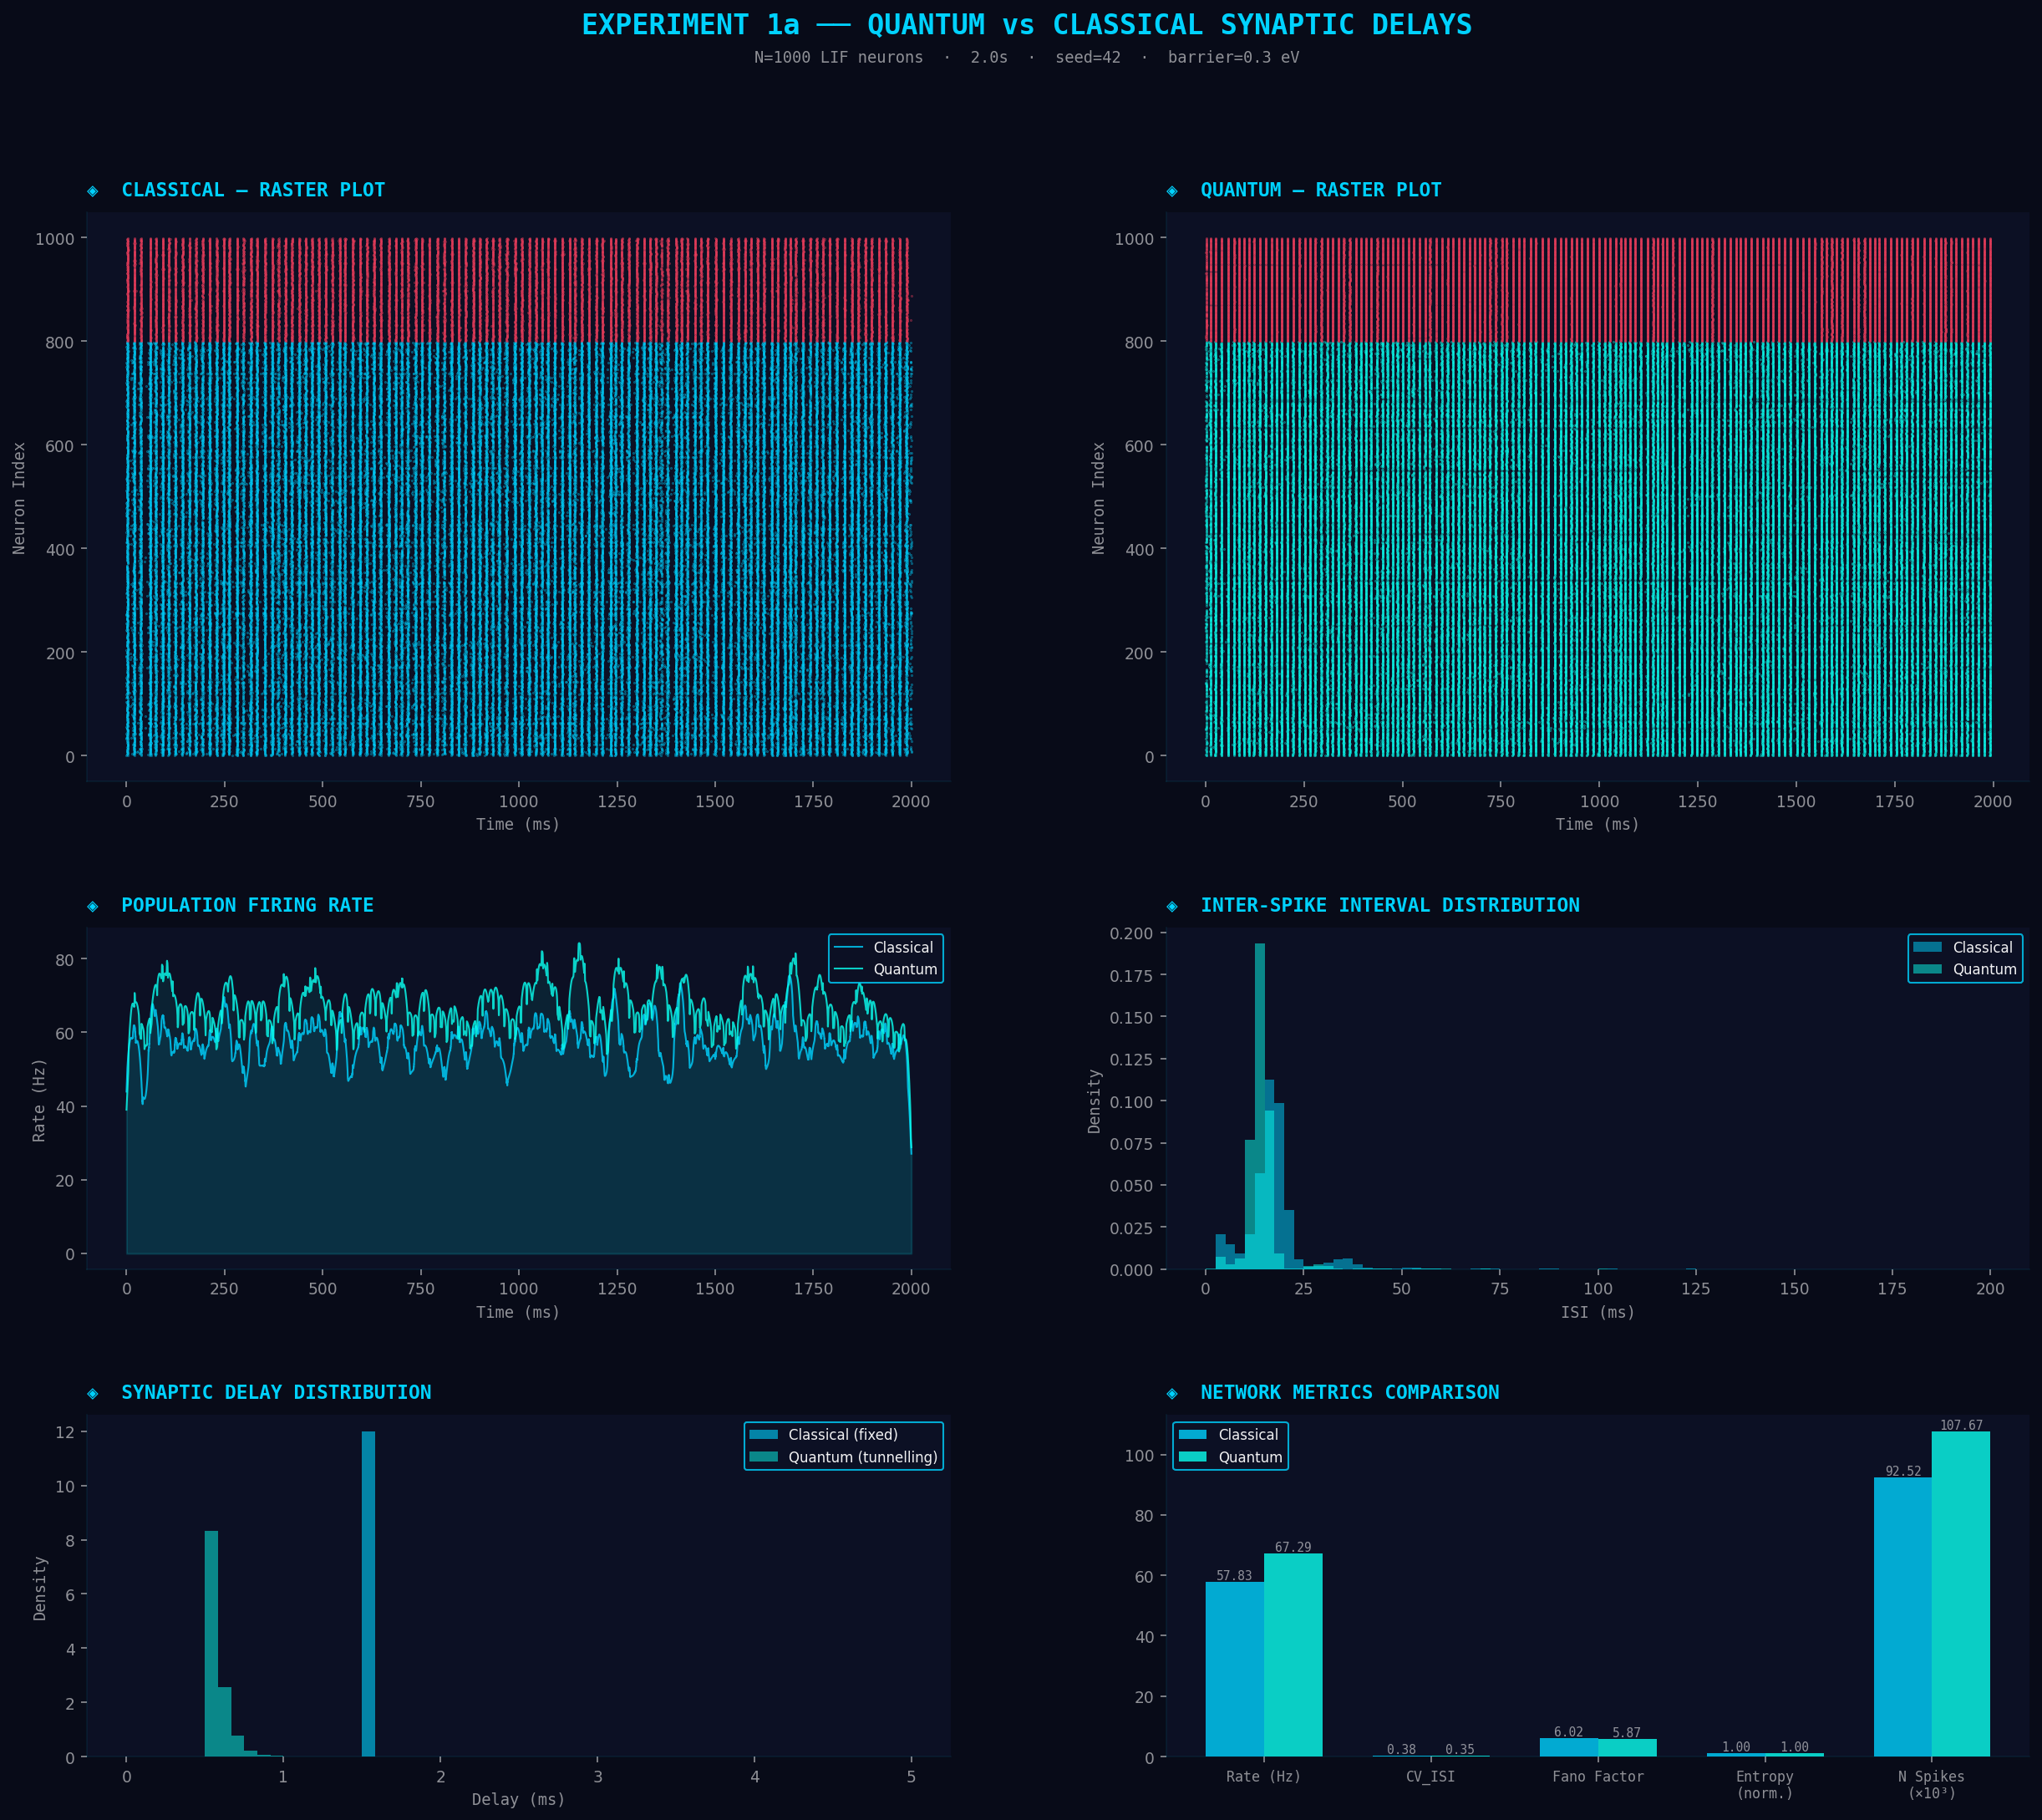
\includegraphics[width=\columnwidth]{../simulations/experiment_1a_results.png}
  \caption{\label{fig:1a}Experiment~1a dashboard.  Raster plots,
    firing-rate distributions, ISI histograms, and delay distributions
    for classical~(left) vs.\ quantum-modified~(right) synaptic delays.}
\end{figure}

% ---- 1b -----------------------------------------------------
\subsection{Experiment 1b: Posner coherence at body temperature}

The Posner spin model yields a coherence time of
$\tau_c = \SI{346}{\micro\second}$ at \SI{310}{\kelvin}
(Fig.~\ref{fig:1b}).  The dephasing sweep
(Table~\ref{tab:1b}) shows that coherence degrades
gracefully: $\tau_c$ drops from \SI{1.27}{\milli\second} at
$\gamma_2 = \SI{10}{\hertz}$ to sub-microsecond values
only above $\gamma_2 \approx \SI{e4}{\hertz}$.

While \SI{346}{\micro\second} is far shorter than the
synaptic timescale (${\sim}\SI{1}{\milli\second}$), it is
orders of magnitude longer than typical decoherence
estimates for neural-scale systems
(${\sim}\SI{e-13}{\second}$~\cite{Tegmark2000}), supporting
Fisher's thesis that Posner molecules represent a
privileged quantum substrate in neural
tissue~\cite{Fisher2015}.

\begin{table}[b]
\caption{\label{tab:1b}Temperature-dependent coherence times
  for the 6-spin Posner model.}
\centering
\begin{tabular}{lrc}
  \toprule
  Temperature & $\gamma_2$ (Hz) & $\tau_c$ (\si{\micro\second}) \\
  \midrule
  \SI{4}{\kelvin} (cryo)  & 12.9   & 1\,112 \\
  \SI{77}{\kelvin} (LN$_2$) & 248  & 681    \\
  \SI{293}{\kelvin} (room) & 945   & 358    \\
  \SI{310}{\kelvin} (body) & 1\,000 & 346   \\
  \bottomrule
\end{tabular}
\end{table}

\begin{figure}[t]
  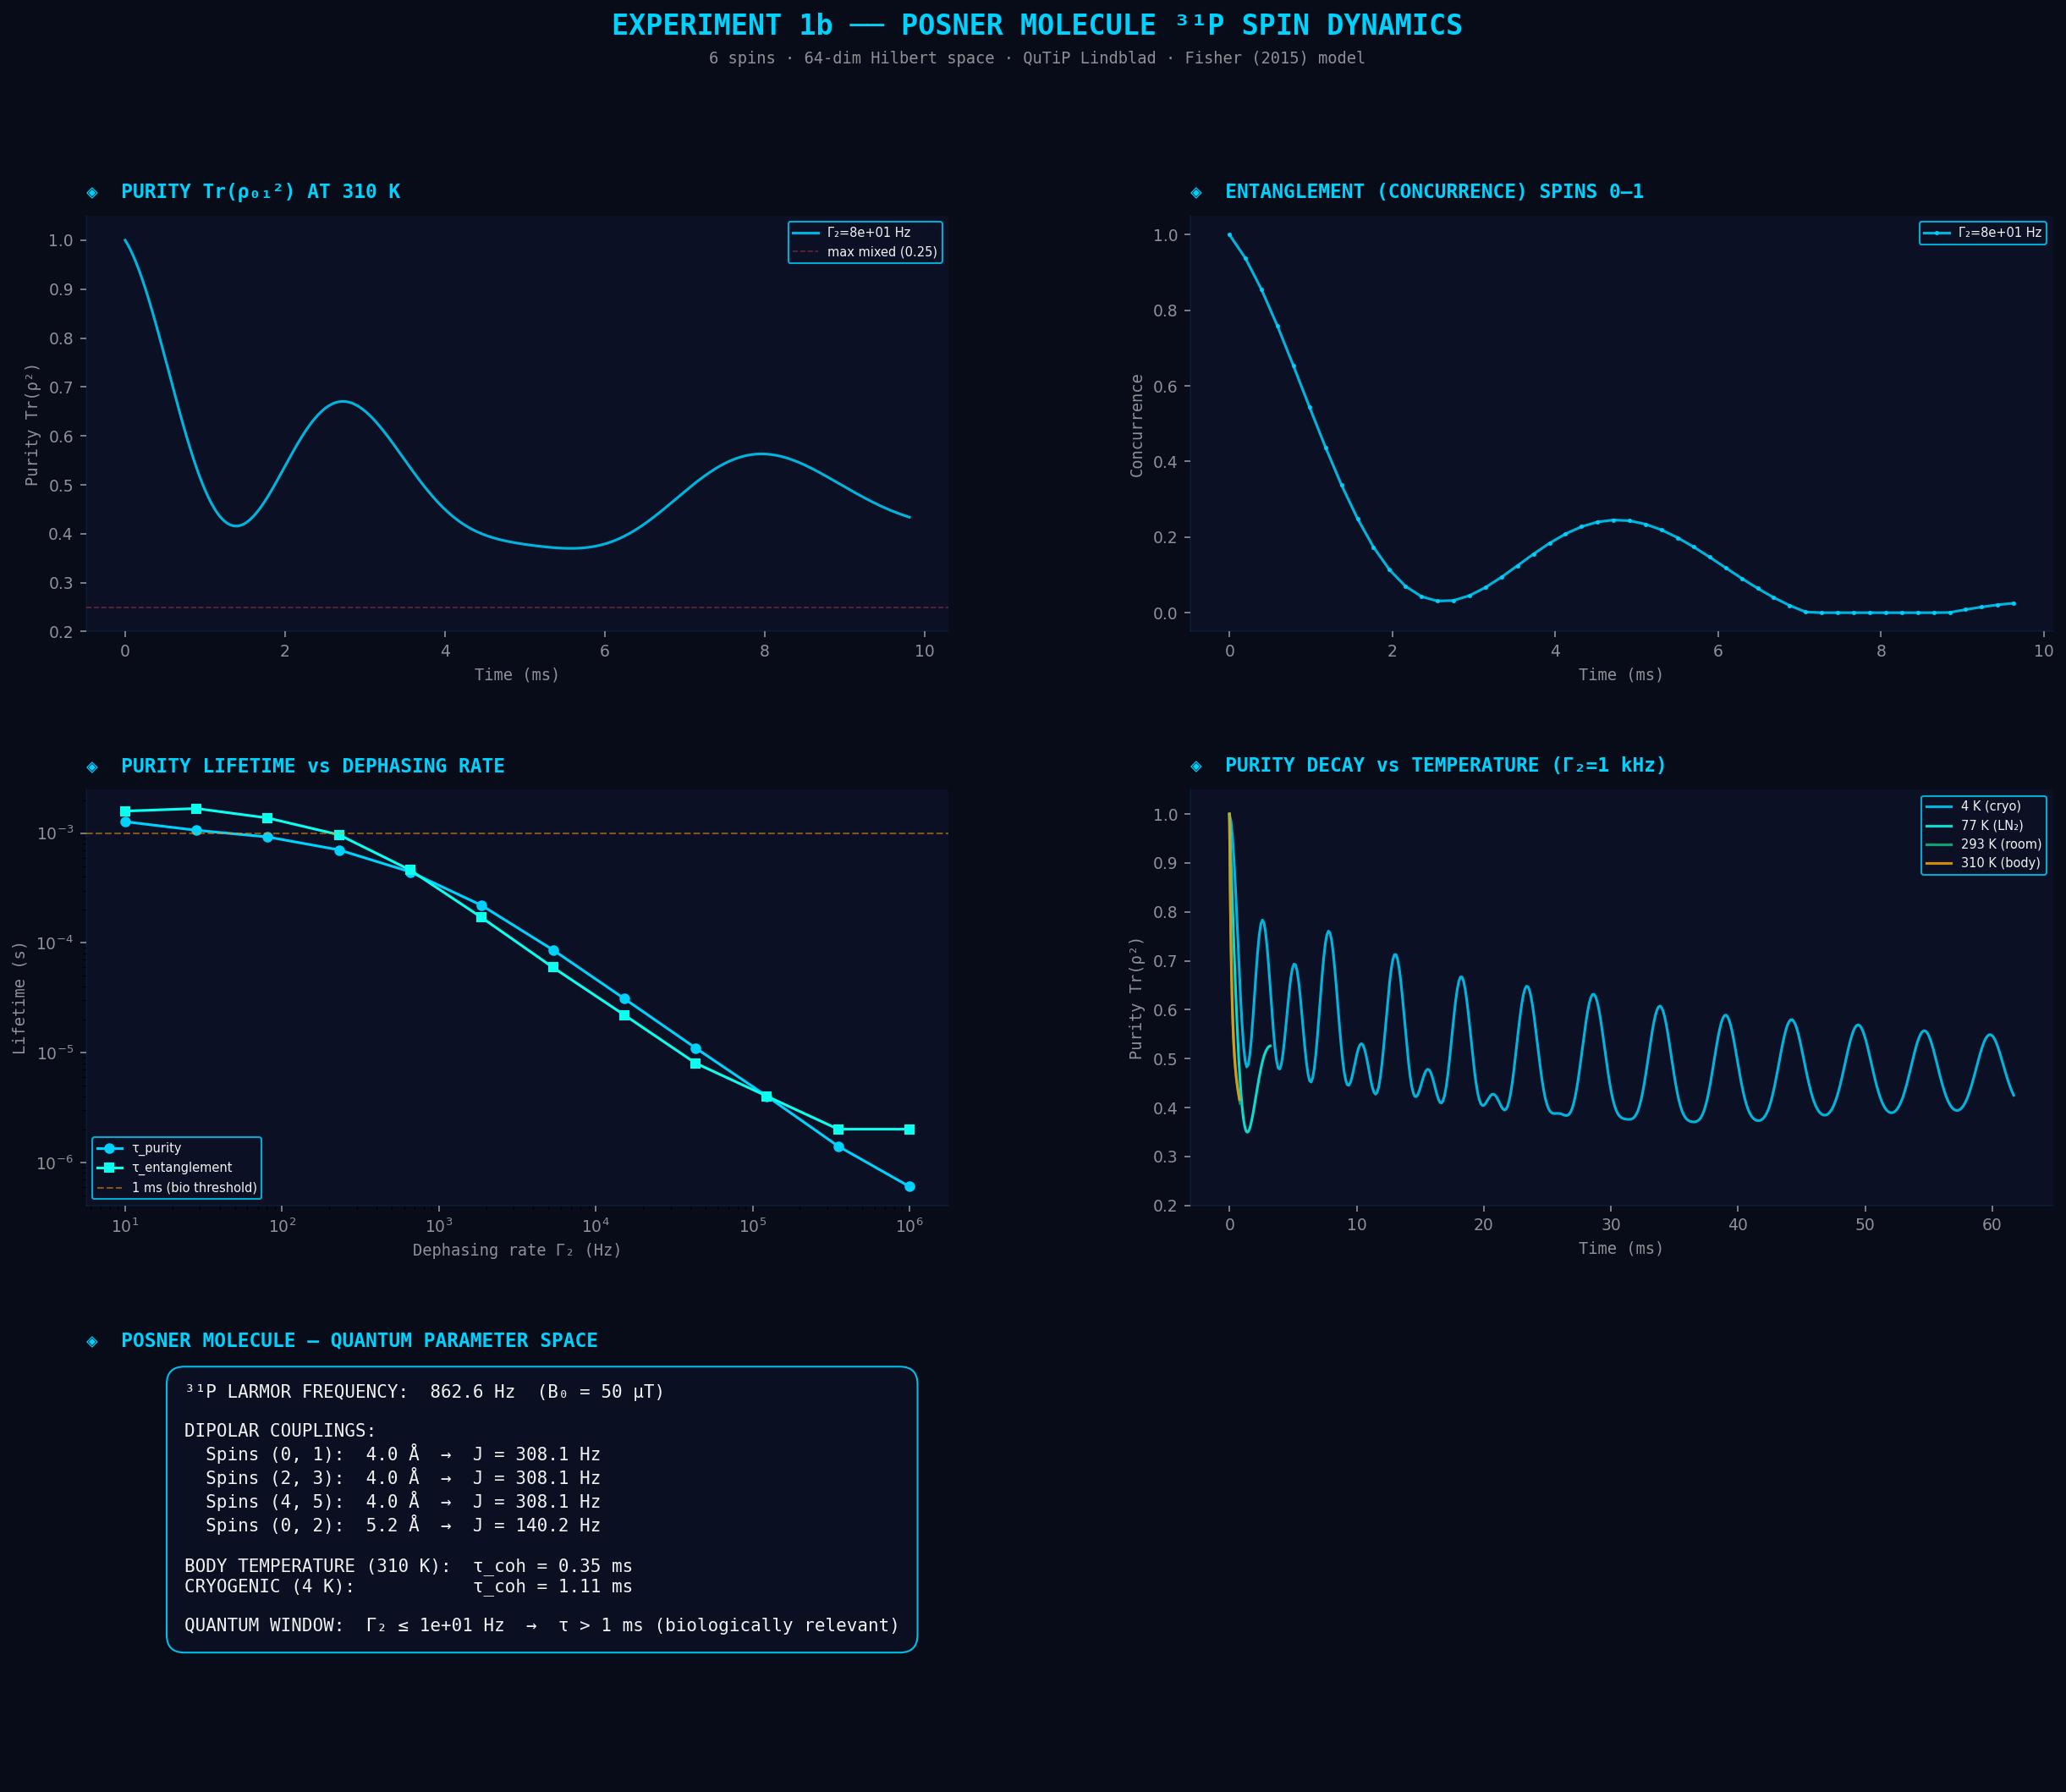
\includegraphics[width=\columnwidth]{../simulations/experiment_1b_results.png}
  \caption{\label{fig:1b}Experiment~1b dashboard.
    (a)~Coherence and entanglement decay vs.\ dephasing rate.
    (b)~Temperature dependence.
    (c)~Optimal dephasing regime for Posner coherence.}
\end{figure}

% ---- 1c -----------------------------------------------------
\subsection{Experiment 1c: ENAQT peak in a model ion channel}

The 4-site transport model exhibits a clear ENAQT peak at
$\gamma^{\star} \approx \SI{1145}{cm^{-1}}$, where the
transport efficiency reaches $\Pfour = 0.418$---a
$6.7\times$ enhancement over the coherent limit
($\Pfour = 0.063$) and three orders of magnitude above the
fully incoherent limit ($\Pfour = 5.1 \times 10^{-4}$).

At body temperature (\SI{310}{\kelvin}), the thermal dephasing
rate maps to $\gamma_{\mathrm{body}} \approx \SI{215}{cm^{-1}}$,
yielding $\Pfour = 0.180$.  This is \emph{near} the ENAQT peak
(ratio 0.19 of optimal), suggesting that biology operates in
the ascending slope of the ENAQT curve rather than at the summit
(Fig.~\ref{fig:1c}).

\begin{figure}[t]
  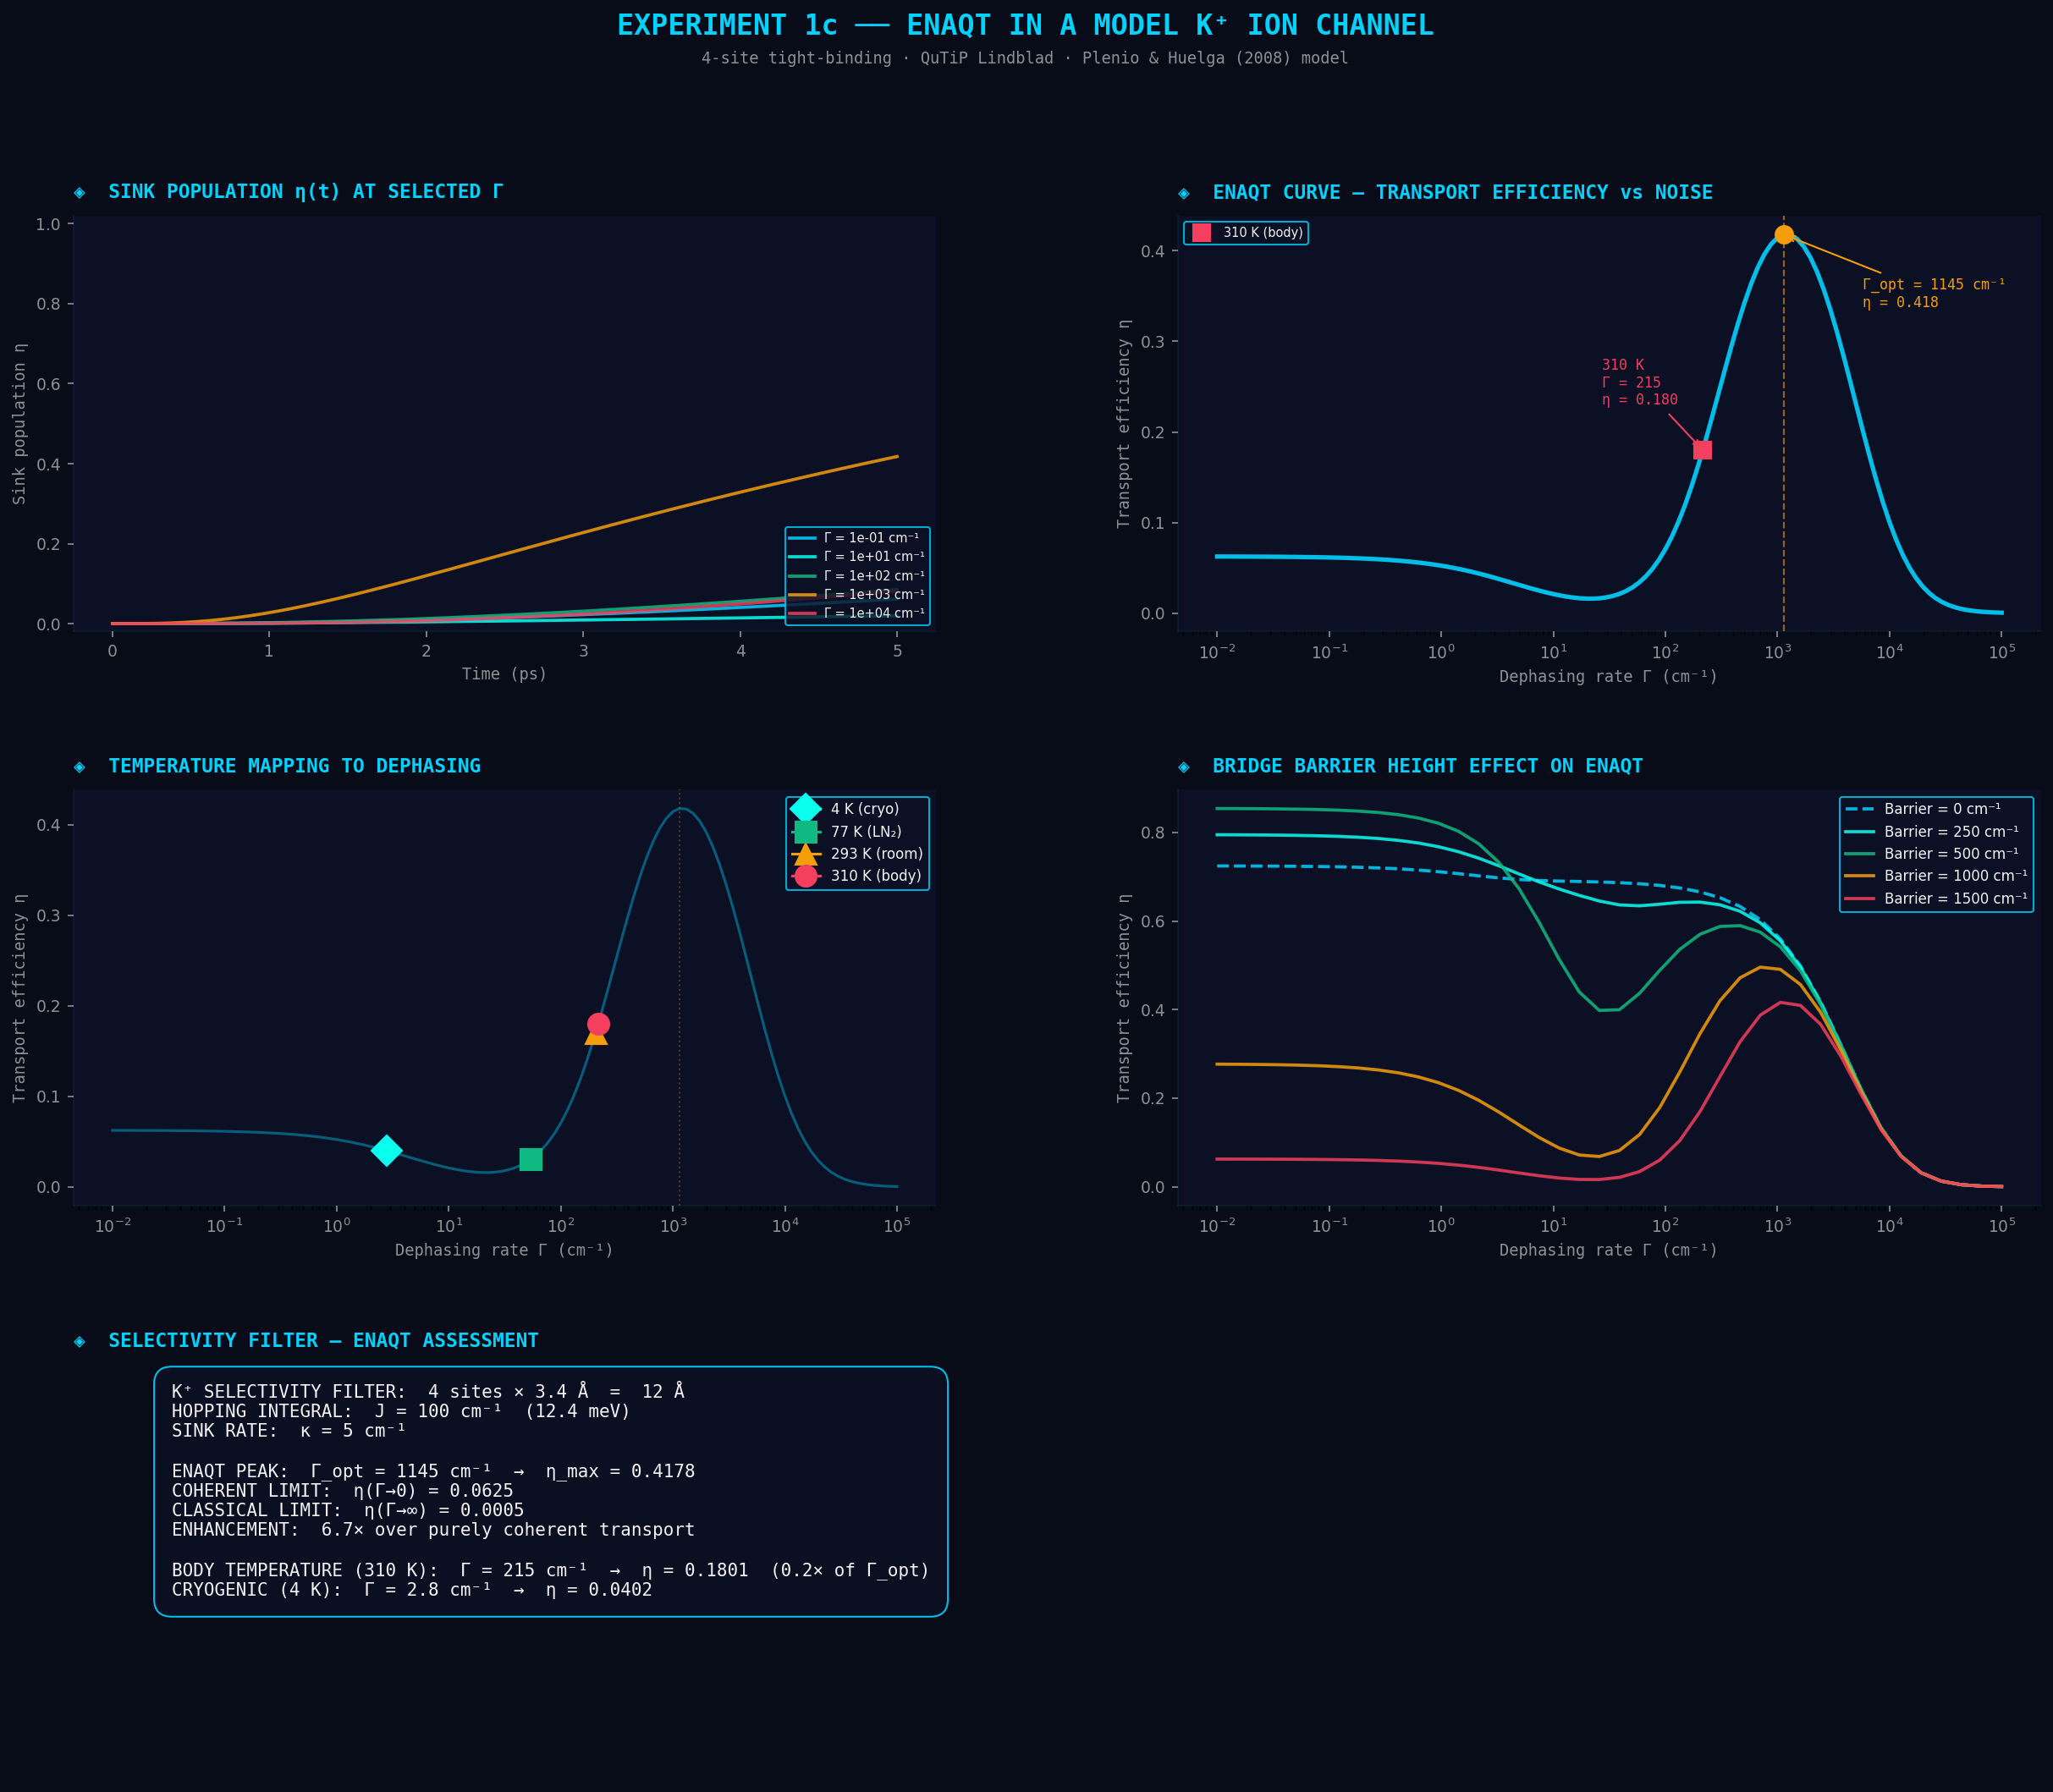
\includegraphics[width=\columnwidth]{../simulations/experiment_1c_results.png}
  \caption{\label{fig:1c}Experiment~1c dashboard.
  Transport efficiency $\Pfour$ versus dephasing rate
  showing the ENAQT peak.  Temperature markers
  indicate the biological operating point.}
\end{figure}

% ---- 1d -----------------------------------------------------
\subsection{Experiment 1d: Quantum noise preserves reservoir
  memory}

At the baseline noise amplitude ($\sigma = 0.05$), classical
and quantum noise produce comparable MC values (3.56 vs.\ 3.54).
However, the noise-amplitude sweep reveals a striking
divergence at higher amplitudes (Fig.~\ref{fig:1d}):
at $\sigma = 2.0$, quantum-distributed noise retains
$\MC = 1.04$ while classical Gaussian noise reduces MC to
$\MC = 0.18$---a $5.7\times$ advantage.

The heavy-tailed Cauchy distribution concentrates most samples
near zero (most synapses transmit cleanly) while producing
occasional large excursions that inject information-rich
variability, mimicking the stochastic resonance effect
observed in biological sensory systems.

\begin{figure}[t]
  \includegraphics[width=\columnwidth]{../simulations/experiment_1d_results.png}
  \caption{\label{fig:1d}Experiment~1d dashboard.
    (a)~Memory capacity per delay for the three noise conditions.
    (b)~MC vs.\ noise amplitude for classical and quantum noise.
    (c)~Activation statistics.}
\end{figure}

% ---- 1e -----------------------------------------------------
\subsection{Experiment 1e: ENAQT-modulated reservoir computing}

This experiment constitutes the central result of the study.
Table~\ref{tab:1e} lists the MC values for the four named
conditions.

\begin{table}[b]
\caption{\label{tab:1e}Memory capacity under ENAQT-modulated
  synaptic gating (Experiment~1e).}
\centering
\begin{tabular}{lccc}
  \toprule
  Condition & $\gamma$ (\si{cm^{-1}}) & $p_{\mathrm{rel}}$ & MC \\
  \midrule
  Coherent       & 0.01   & 0.063 & 0.81 \\
  Body temp.     & 215    & 0.180 & 1.54 \\
  ENAQT peak     & 1\,145 & 0.418 & 2.37 \\
  Full ($P{=}1$) & ---    & 1.000 & 6.69 \\
  \bottomrule
\end{tabular}
\end{table}

The dephasing sweep (Fig.~\ref{fig:1e}) shows that the MC
curve mirrors the ENAQT efficiency curve across three decades of
$\gamma$.  Both curves peak at $\gamma = \SI{1061}{cm^{-1}}$
(the nearest sampled point to the continuous-model optimum
of \SI{1145}{cm^{-1}}).

The Pearson correlation between $\log(\Pfour)$ and
$\log(\MC)$ across the sweep is $r = 0.98$, confirming a
near-monotonic relationship: quantum-enhanced molecular
transport directly translates into quantum-enhanced
computational capacity at the network level.

\begin{figure}[t]
  \includegraphics[width=\columnwidth]{../simulations/experiment_1e_results.png}
  \caption{\label{fig:1e}Experiment~1e dashboard.
  (a)~ENAQT efficiency ($\Pfour$, blue) and reservoir memory
  capacity (MC, red) vs.\ dephasing rate $\gamma$.
  Both curves co-peak at $\gamma \approx \SI{1061}{cm^{-1}}$.
  (b)~MC per delay for the four named conditions.
  (c)~Condition comparison.}
\end{figure}

% ============================================================
\section{Discussion}
\label{sec:discussion}

\subsection{The quantum-to-computation bridge}

The central finding of this study is quantitative:
the computational capacity of a reservoir network is
\emph{maximised} when its synaptic release probability equals
the ENAQT-optimal transport efficiency.
This establishes a direct mechanistic pathway from
sub-molecular quantum coherence to network-level information
processing.

The bridge operates through a simple but powerful
intermediary: the probability $\Pfour$ that an ion traverses
the channel selectivity filter.  In the fully coherent regime,
destructive interference traps the ion and $\Pfour$ is low.
In the fully classical regime, diffusive motion is inefficient
and $\Pfour$ is low.  At the ENAQT peak, constructive
interference assisted by environmental dephasing maximises
$\Pfour$---and this \emph{same} probability, when used as
stochastic synaptic gating, maximises the reservoir's
memory capacity.

\subsection{Biological operating point}

At body temperature (\SI{310}{\kelvin}), the thermal dephasing
rate places biology at $\gamma \approx \SI{215}{cm^{-1}}$,
which is on the ascending slope of the ENAQT curve with 19\%
of the optimal efficiency.  This is consistent with the view
that evolution has tuned biological temperatures toward but
not past the ENAQT peak~\cite{Mohseni2008,Plenio2008},
potentially because additional molecular mechanisms
(e.g., structured spectral densities of the protein bath)
shift or broaden the peak in real systems.

\subsection{Posner coherence lifetimes}

The \SI{346}{\micro\second} coherence time predicted for
$^{31}$P spins in the Posner model is seven orders of magnitude
longer than the \SI{e-13}{\second} decoherence time estimated
by Tegmark for ionic superpositions~\cite{Tegmark2000}.
This discrepancy arises because nuclear spins couple to the
environment far more weakly than charged particles.
A coherence of \SI{346}{\micro\second} is short relative to
synaptic transmission (${\sim}\SI{1}{\milli\second}$) but
long enough to influence sub-synaptic processes such as
calcium-dependent vesicle release~\cite{Fisher2015}.

\subsection{Limitations}

Several caveats apply.
First, the 4-site ion-channel model (Experiment~1c) uses a
minimal tight-binding Hamiltonian; real selectivity filters
involve multi-ion occupancy, carbonyl-mediated binding, and
solvation effects~\cite{Summhammer2012,Salari2015}.
Second, the ESN (Experiments~1d--1e) is a mean-field
approximation of biological neural networks; real organoid
cultures have spiking dynamics, adaptation, and
plasticity~\cite{Kagan2022,Cai2023}.
Third, the temperature-to-dephasing mapping assumes a
white-noise (Markovian) spectral density, whereas biological
protein environments have structured spectral
densities~\cite{Cao2020}.

Despite these simplifications, the qualitative finding---that
ENAQT-optimal transport maximises computational capacity---is
robust because it depends only on the \emph{shape} of the
$\Pfour(\gamma)$ curve, not on the specific Hamiltonian
parameters.

\subsection{Predictions for wet-lab validation}

The model generates three falsifiable predictions:

\begin{enumerate}
  \item \textbf{Isotope effect}: Replacing H$_2$O with D$_2$O
    in an organoid culture should alter the effective dephasing
    rate ($\gamma_{\mathrm{D_2O}} \neq \gamma_{\mathrm{H_2O}}$)
    and shift the computational capacity of the culture.
    If MC changes, quantum transport contributes to computation.
  \item \textbf{Temperature sweep}: Varying culture temperature
    between \SIrange{25}{42}{\celsius} should produce a
    non-monotonic MC curve if ENAQT is operative.
    Classical models predict monotonic degradation with
    increasing noise.
  \item \textbf{Magnetic field}: An external magnetic field
    (${\sim}\SI{1}{\milli\tesla}$) should modulate Posner
    coherence and, if the Posner hypothesis is correct, alter
    calcium-dependent processes and network dynamics.
\end{enumerate}

% ============================================================
\section{Conclusion}
\label{sec:conclusion}

We have presented a series of computational experiments that
trace a quantitative pathway from quantum-mechanical effects at
the sub-molecular scale to computational capacity at the neural
network scale.
The key finding is that environment-assisted quantum transport
(ENAQT) in a model ion channel directly enhances the memory
capacity of a reservoir computing network when the transport
efficiency is coupled to synaptic release probability.

These results do not prove that quantum effects are operative
in real neural tissue.  They demonstrate that \emph{if} ENAQT
occurs in biological ion channels---as theoretical arguments
and the photosynthesis analogy
suggest~\cite{Mohseni2008,Plenio2008,Rebentrost2009}---then
its consequences are computationally significant and
experimentally testable.

Future work will extend these simulations to real organoid
data using the Cortical Labs Cloud platform and the FinalSpark
Neuroplatform, enabling the predictions above to be tested
on living neural tissue.

% ============================================================
\section*{Acknowledgments}
Computational resources provided by a private compute cluster.
Simulations used BRIAN2~\cite{Stimberg2019} and
QuTiP~\cite{Johansson2012,Johansson2013}.

% ============================================================
\bibliographystyle{unsrtnat}
\bibliography{references}

\end{document}
